\documentclass{hw_template}

\usepackage{arydshln}

\title{\bfseries Домашня Робота \#3 з Теорії Коливань}
\author{\bfseries Захаров Дмитро}
\date{16 березня, 2025}

\begin{document}

\pagestyle{fancy}

\maketitle

\section{Задача 1(б)}


\begin{problem}
    Визначте період вільних коливань вантажу маси $m$, прикріпленого до двох пружин 
    з жорсткостями $k_1$ та $k_2$, які з'єднанні послідовно.
\end{problem}

\textbf{Розв'язання.} Нехай до пружин прикладена сила $F$, причому перша 
пружина розтягнулася на $x_1$, а друга на $x_2$. Оскільки з'єднання 
послідовне, то сила, яка діє на першу пружину, дорівнює силі, яка діє
на другу пружину, а загальне розтягнення $x$ дорівнює сумі розтягнень
пружин: $x = x_1 + x_2$. Таким чином, якщо позначити ``ефективну''
жорсткість системи як $k$, то маємо:
\begin{equation*}
    F = k_1x_1 = k_2x_2 = k(x_1+x_2)
\end{equation*}

Звідси маємо $x_1=F/k_1$ та $x_2=F/k_2$, тому ефективна жорсткість:
\begin{equation*}
    k = \frac{F}{x_1+x_2} = \frac{F}{\frac{F}{k_1} + \frac{F}{k_2}} = \frac{k_1k_2}{k_1+k_2}
\end{equation*}

Період коливань в такому разі:
\begin{equation*}
    T = 2\pi\sqrt{\frac{m}{k}} = 2\pi\sqrt{\frac{m(k_1+k_2)}{k_1k_2}}
\end{equation*}

\newpage

\section{Задача 2}

\begin{problem}
    Визначте період малих коливань однорідного циліндра з діаметром $d$ і масою
$m$, прикріпленого до двох пружин жорсткості $k$, як показано на рисунку.
Циліндр котиться без ковзання по горизонтальній поверхні.
\end{problem}

\begin{center}
    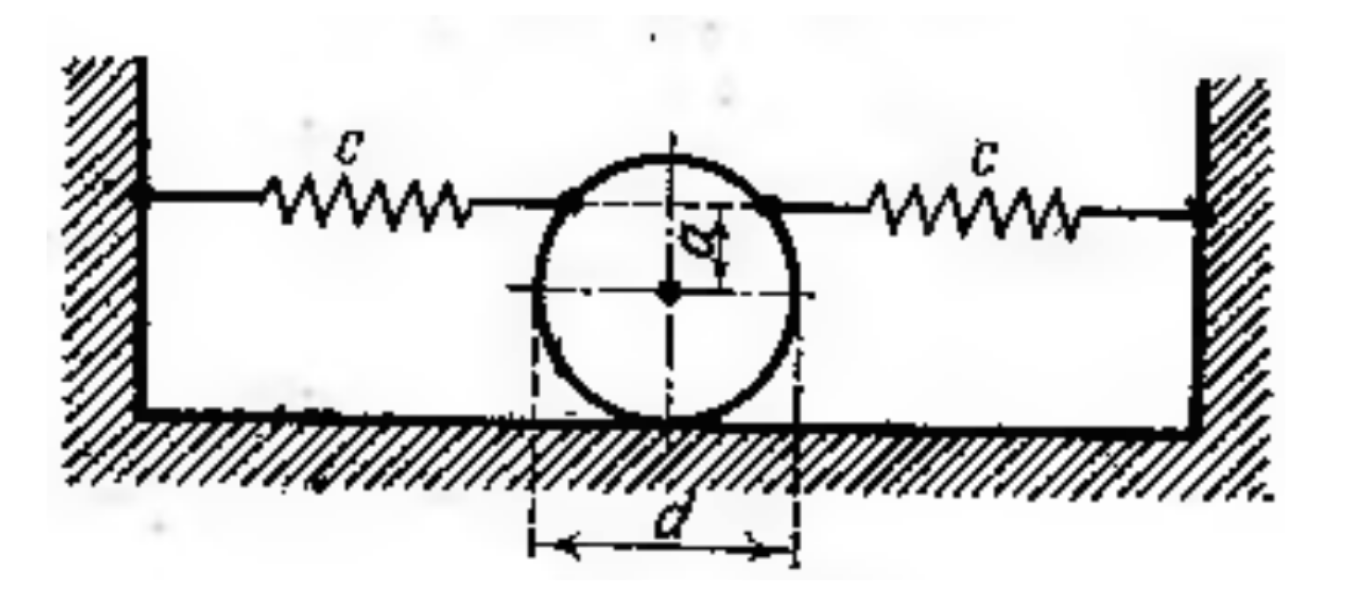
\includegraphics[width=0.5\linewidth]{images/hw_3_problem_3.png}
\end{center}

\textbf{Розв'язання.} У якості координати, що описує систему, виберемо кут
$\theta$, на який відхиляється циліндр від вертикалі. Запишемо потенціальну та
кінетичну енергію системи у разі малого відхилення $\theta \ll 1$.

Потенціальна енергія складається з енергії розтягнення пружин. Прослідкуємо,
як саме змінюється довжина пружин. Введемо систему координат наступним чином: 
центр знаходиться у центрі циліндра, вісь $Ox$ спрямована праворуч, 
$Oy$ вгору. Запишемо координати кінців пружин (лівого кінця $K_L$ та правого 
$K_R$). Врахуємо, що лівий кінець $K_R$ відхилений на кут $\theta_R=\theta$ до $Ox$, 
а $K_L$ в свою чергу на кут $\theta_L=\pi-\theta$.
\begin{equation*}
    K_R = \left(\frac{d}{2}\cos\theta_0, \frac{d}{2}\sin\theta_0\right), \quad 
    K_L = \left(\frac{d}{2}\cos\left(\pi-\theta_0\right), \frac{d}{2}\sin(\pi-\theta_0)\right), \quad
    \sin\theta_0 = \frac{a}{d/2}
\end{equation*}

Запишемо нові координати кінців пружин після відхилення на кут $\theta$:
\begin{equation*}
    K_R' = \left(\frac{d}{2}\cos(\theta_0+\theta)-\frac{d}{2}\theta, \frac{d}{2}\sin(\theta_0+\theta)\right), 
    \; K_L' = \left(\frac{d}{2}\cos(\pi-\theta_0+\theta)-\frac{d}{2}\theta, \frac{d}{2}\sin(\pi-\theta_0+\theta)\right)
\end{equation*}

Зміна довжин пружин: це довжини $\Delta x_L = K_LK_L'$ та $\Delta x_R
= K_RK_R'$. Почнемо з $\Delta x_L$:
\begin{equation*}
    (\Delta x_L)^2 = \frac{d^2}{4}\left(\cos(\theta_0+\theta)-\cos\theta_0 + \theta\right)^2 + \frac{d^2}{4}\left(\sin(\theta_0+\theta) - \sin\theta_0\right)^2
\end{equation*}

Розглянемо малу зміну $\cos(\theta_0+\theta)-\cos\theta_0$ та $\sin(\theta_0+\theta)-\sin\theta_0$
\begin{align*}
    \cos(\theta_0+\theta) - \cos \theta_0 &= \cos\theta_0\cos\theta - \sin\theta_0\sin\theta - \cos\theta_0 \\
    &\approx \left(1-\frac{\theta^2}{2}\right)\cos\theta_0 - \sin\theta_0 \cdot \theta - \cos\theta_0  
    = -\frac{\theta^2}{2}\cos\theta_0 - \theta\sin\theta_0 \\
    \sin(\theta_0+\theta) - \sin \theta_0 &= \sin\theta_0\cos\theta + \cos\theta_0\sin\theta - \sin\theta_0 \\
    &\approx \left(1-\frac{\theta^2}{2}\right)\sin\theta_0 + \cos\theta_0 \cdot \theta - \sin\theta_0 
    = -\frac{\theta^2}{2}\sin\theta_0 + \theta\cos\theta_0
\end{align*}

Отже, можемо знайти зміну довжини. Розглянемо вираз $((\cos(\theta_0+\theta)-\cos\theta_0)+\theta)^2$:
\begin{align*}
    ((\cos(\theta_0+\theta)-\cos\theta_0)+\theta)^2 &= (\cos(\theta_0+\theta)-\cos\theta_0)^2 - 2\theta(\cos(\theta_0+\theta)-\cos\theta_0) + \theta^2 \\
    &\approx \left(\frac{\theta^2}{2}\cos\theta_0 - \theta\sin\theta_0\right)^2 + 2\theta\left(\frac{\theta^2}{2}\cos\theta_0 + \theta\sin\theta_0\right) + \theta^2 \\
    &\approx \theta^2\sin^2\theta_0 + 2\theta^2\sin\theta_0 + \theta^2 = \theta^2(1+\sin\theta_0)^2 = \theta^2\left(1+\frac{2a}{d}\right)^2
\end{align*}

Зміна вертикальної компоненти:
\begin{equation*}
    (\sin(\theta_0+\theta) - \sin\theta_0)^2 = \left(-\frac{\theta^2}{2}\sin\theta_0 + \theta\cos\theta_0\right)^2 \approx \theta^2\cos^2\theta_0
\end{equation*}

Таким чином, квадрат зміщення:
\begin{equation*}
    (\Delta x_L)^2 = \frac{d^2\theta^2}{4}\left(1+\frac{2a}{d}\right)^2 + \frac{d^2\theta^2}{4}\cos^2\theta_0 = \frac{d^2\theta^2}{4}\left(1+\frac{4a}{d}+\frac{4a^2}{d^2} + 1 - \frac{4a^2}{d^2}\right) = \frac{d^2\theta^2}{2}\left(1+\frac{2a}{d}\right)
\end{equation*}

З геометричних міркувань, можна вважати $\Delta x_L \approx \Delta x_R =: \Delta x$.

Таким чином, зміна потенціальної енергії:
\begin{equation*}
    V(\theta) = 2 \cdot \frac{1}{2}k(\Delta x)^2 = \frac{1}{2}kd^2\left(1+\frac{2a}{d}\right)\theta^2
\end{equation*}

Запишемо вираз для кінетичної енергії. Вона складається з кінетичної енергії
процесу обертання циліндра та кінетичної енергії руху центру мас циліндра:
\begin{equation*}
    T = \frac{1}{2}I\dot{\theta}^2 + \frac{1}{2}m\left(\frac{d}{2}\dot{\theta}\right)^2
\end{equation*}

Момент інерції цільного циліндру відносно його центру мас: $I =
\frac{1}{2}m\left(\frac{d}{2}\right)^2 = md^2/8$. Таким чином, кінетична
енергія:
\begin{equation*}
    T = \frac{1}{2}m\left(\frac{d^2}{8}\dot{\theta}^2 + \frac{d^2}{4}\dot{\theta}^2\right) = \frac{3md^2\dot{\theta}^2}{16}
\end{equation*}

Отже, загальна енергія системи:
\begin{equation*}
    E = T + V = \frac{3}{16}md^2\dot{\theta}^2 + \frac{1}{2}k d^2\left(1+\frac{2a}{d}\right)\theta^2
\end{equation*}

Звідси можна одразу знайти циклічну частоту коливань. Дійсно, енергія має вираз
$E(\theta) =
\frac{1}{2}\widetilde{k}\theta^2+\frac{1}{2}\widetilde{m}\dot{\theta}^2$ з
ефективною ``жорсткістю'' $\widetilde{k}$ та ``масою'' $\widetilde{m}$, де:
\begin{equation*}
    \widetilde{k} = k d^2 \left(1+\frac{2a}{d}\right), \quad \widetilde{m} = \frac{3md^2}{8}
\end{equation*}

Отже, циклічна частота:
\begin{equation*}
    \omega^2 = \frac{\widetilde{k}}{\widetilde{m}} = \frac{8k}{3m}\left(1+\frac{2a}{d}\right)
\end{equation*}

Звідси період коливань:
\begin{equation*}
    T = \pi\sqrt{\frac{3m}{2k\left(1+\frac{2a}{d}\right)}}
\end{equation*}

\newpage
\section{Задача 4}
\begin{problem}
    Визначте період малих коливань у вертикальній площині фізичного маятника,
який складається з двох стержнів з масами $m$ і $2m$ та довжинами $\ell$ і
$2\ell$ відповідно. Стержні прикріплені один до одного під прямим кутом.
\end{problem}

\begin{center}
    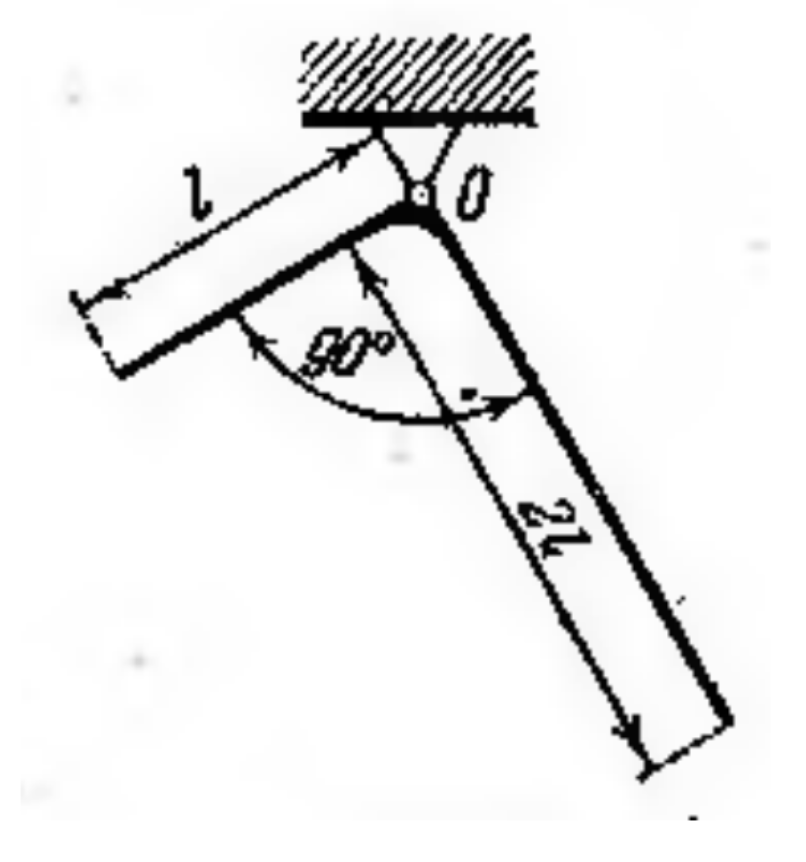
\includegraphics[width=0.3\linewidth]{images/hw_3_problem_4.png}
\end{center}

\textbf{Розв'язання.} Спочатку знайдемо момент інерції системи. Момент інерції
стержня довжиною $\ell$ відносно його кінцю дорівнює $I = \frac{1}{3}m\ell^2$.
В нашому випадку маємо:
\begin{equation*}
    I = \frac{1}{3}m\ell^2 + \frac{1}{3}(2m)(2\ell)^2 = \frac{1}{3}m\ell^2 + \frac{8}{3}m\ell^2 = 3m\ell^2
\end{equation*}

Тепер знайдемо положення рівноваги системи. Нехай кут відхилення від вертикалі
правого стержня дорівнює $\theta$. Тоді кут відхилення від вертикалі лівого
стержня дорівнює $\varphi = \frac{\pi}{2}-\theta$. В положені рівноваги,
центр мас системи має лежати під точкою підвісу. Таким чином, можемо записати
рівняння рівноваги:
\begin{equation*}
    2m \cdot \ell \sin \theta = m \cdot \frac{\ell}{2}\sin\varphi \Rightarrow \sin\varphi = 4\sin\theta
\end{equation*}

Оскільки $\sin\varphi = \cos\theta$, то $\cos\theta = 4\sin\theta$ або
$\tan\theta = \frac{1}{4}$. Звідси $\sin\theta=\frac{1}{\sqrt{17}}$ та 
$\cos\theta = \frac{4}{\sqrt{17}}$.

Знайдемо висоту центра мас системи $h$ від точки підвісу. Маємо:
\begin{align*}
    h &= \frac{1}{3m}\left(\frac{m\ell}{2}\cos\varphi + 2m\ell \cos \theta\right)
    = \frac{1}{6}\ell\sin\theta + \frac{2}{3}\ell \cos\theta \\ 
    &= \frac{1}{6}\ell \cdot \frac{1}{\sqrt{17}} + \frac{2}{3}\ell \cdot \frac{4}{\sqrt{17}} \\
    &= \frac{\sqrt{17}}{6}\ell
\end{align*}

Таким чином, маємо фізичний маятник маси $3m$ з моментом інерції $I = 3m\ell^2$ та
висотою центра мас $h = \frac{\sqrt{17}}{6}\ell$. Циклічна частота коливань:
\begin{equation*}
    \omega^2 = \frac{3mgh}{I} = \frac{\frac{\sqrt{17}}{2}mg\ell}{3m\ell^2} = \frac{\sqrt{17}}{6} \frac{g}{\ell}
\end{equation*}

Звідси період коливань $T=2\pi\sqrt{6\ell/\sqrt{17}g}$.


\end{document}